%**************************************************************************************
% License:
% CC BY-NC-SA 4.0 (http://creativecommons.org/licenses/by-nc-sa/4.0/)
%**************************************************************************************

\documentclass[beamer]{beamer}

\mode<presentation> {

\usetheme{Madrid}

% Burnt orange
\definecolor{burntorange}{rgb}{0.8, 0.33, 0.0}
\colorlet{beamer@blendedblue}{burntorange}
% Pale yellow
\definecolor{paleyellow}{rgb}{1.0, 1.0, 0.953}
\setbeamercolor{background canvas}{bg=paleyellow}
% Secondary and tertiary palett
\setbeamercolor*{palette secondary}{use=structure,fg=white,bg=burntorange!80!black}
\setbeamercolor*{palette tertiary}{use=structure,fg=white,bg=burntorange!60!black}

% To remove the footer line in all slides uncomment this line
%\setbeamertemplate{footline}
% To replace the footer line in all slides with a simple slide count uncomment this line
%\setbeamertemplate{footline}[page number]

% To remove the navigation symbols from the bottom of all slides uncomment this line
%\setbeamertemplate{navigation symbols}{}
}

\usepackage{amsmath}
\usepackage{bm}
\usepackage{breqn}
\usepackage{graphicx} % for figures
\usepackage{subcaption} % for subplots 
\usepackage[labelsep=space,tableposition=top]{caption}
\renewcommand{\figurename}{Fig.} 
\usepackage{cleveref}
\usepackage{caption,subcaption}% http://ctan.org/pkg/{caption,subcaption}
\usepackage{booktabs} % Allows the use of \toprule, \midrule and \bottomrule in tables

%----------------------------------------------------------------------------------------
%	TITLE PAGE
%----------------------------------------------------------------------------------------
% The short title appears at the bottom of every slide, the full title is only on the title page
\title[CE394M: 1D - FEM]{CE394M: 1D-Finite Element Method} 
\author{Krishna Kumar} % name
\institute[UT Austin] % institution 
{
University of Texas at Austin \\
\medskip
\textit{
  \url{krishnak@utexas.edu}} % Your email address
}
\date{\today} % Date, can be changed to a custom date

\begin{document}

\begin{frame}
\titlepage % title page as the first slide
\end{frame}

\begin{frame}
 % Table of contents slide, comment this block out to remove it
 \frametitle{Overview}
 % Throughout your presentation, if you choose to use \section{} and \subsection{} 
 % commands, these %will automatically be printed on this slide as an overview 
 \tableofcontents
\end{frame}

%----------------------------------------------------------------------------------------
% slides
%----------------------------------------------------------------------------------------
\section{FEM workflow}
%------------------------------------------------
\begin{frame}
\frametitle{Finite Element Analysis}
\begin{figure}[ht]
	\centering
	\includegraphics[width=\textwidth]{figs/fem.png}
\end{figure}
\end{frame}

%------------------------------------------------
\begin{frame}
\frametitle{Finite Element Analysis}
FEM is a systematic procedure for approximating differential equations. For any problem in any spatial dimension it follows the same steps:
\mode<beamer>{
\begin{enumerate}
\item Identify the equation of interest
\item Cast the equation of interest in a weak form
\item Select a finite element type
\item Construct the element matrix and vector
\item Assemble the global matrix and vector and apply boundary conditions
\item Solve the system of linear equations
\end{enumerate}
}
\mode<handout>{
\vspace{5cm}
}
\end{frame}

%---------------------------------------------------
\section{1D FEM}
%------------------------------------------------
\begin{frame}
\frametitle{1D Finite Element Analysis of a cantilever beam}
\begin{figure}[ht]
	\centering
	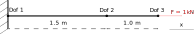
\includegraphics[width=\textwidth]{figs/cantilever.png}
	\caption*{1D cantilever beam}
\end{figure}
Assume $L$ as unit length $L = 1$. Unit force $f = 1$.
\end{frame}

%------------------------------------------------
\begin{frame}
\frametitle{1D Finite Element Analysis of a cantilever beam}
What element should be used?
\begin{figure}[ht]
	\centering
	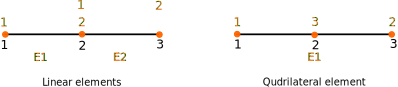
\includegraphics[width=\textwidth]{figs/fem-cantilever-linear-quad.png}
	\caption*{1D discretization of a cantilever beam}
\end{figure}
\end{frame}

%------------------------------------------------
\begin{frame}
\frametitle{1D FEM: Shape functions and derivatives}
Shape function $\mathbf{N}$:
\mode<beamer>{
	\begin{align*}
		N_1(x) & = -\frac{x}{L} + 1 \\
		N_2(x) & = \frac{x}{L}
	\end{align*}
	\begin{align*}
		N_1(x) & = -x + 1 \\
		N_2(x) & = x
	\end{align*}
}
\mode<handout>{
	\vspace{2.5cm}
}
$\mathbf{B}$ is the derivatives of the shape functions:
\mode<beamer>{
	\begin{equation*}
		\mathbf{B} = \left[\frac{dN_1(x)}{dx} \quad \frac{dN_2(x)}{dx}\right]
	\end{equation*}
	
	\begin{equation*}
		\mathbf{B} = \left[\frac{-1}{L} \quad \frac{1}{L}\right]  = \left[-1 \quad 1\right]
	\end{equation*}
}
\mode<handout>{
	\vspace{2.5cm}
}
\end{frame}


%------------------------------------------------
\begin{frame}
\frametitle{1D FEM: Stiffness and force}
Element stiffness $k_e$:
\mode<beamer>{
	\begin{equation*}
		k_e = \int \textbf{B}^T EA \, B\, \mathrm{d}x
	\end{equation*}
	\begin{equation*}
		k_e = 
		\begin{bmatrix}
		 1 & -1 \\
		-1 &  1 \\
		\end{bmatrix}
	\end{equation*}
}
\mode<handout>{
	\vspace{2.5cm}
}
Right-hand side vector $b_e$ is:
\mode<beamer>{
	\begin{equation*}
	b_e = \int N^T \, f\, \mathrm{d}x = \int_0^L 	\begin{bmatrix}
	-\frac{x}{L} + 1\\
	\frac{x}{L}\\
	\end{bmatrix}
	\end{equation*}
	
	\begin{equation*}
		b_e =
		\begin{bmatrix}
			-\frac{1}{2}\\
			\frac{1}{2}\\
		\end{bmatrix}
	\end{equation*}
}
\mode<handout>{
	\vspace{2.5cm}
}
\end{frame}

\end{document} 


